\chapter{Representación y visualización de superficies implícitas}

Escribir introducción.

\section{Representación de superficies algebraicas y blobs}

\subsection{Superficies algebraicas}

Una superficie se dice algebraica si se define por polinomios cuyo grado indica el grado de la superficie. El grado indica el número de intersecciones de la superficie y una recta.\cite{Bloomenthal97} Por ejemplo un plano tiene grado 1 mientras que una esfera tiene grado 2. El uso de polinomios tiene la ventaja de ser menos costoso, en tiempo de renderización, que cualquier otra representación analítica general.
\par Las superficies algebraicas más comunes son las cuadráticas. Este tipo de superficies son fáciles de renderizar son muy pocos parámetros para controlar su forma, además, es posible usar coordinadas homogéneas para aplicar transformaciones afines. A continuación mostramos típicas superficies cuadráticas como son la esfera, el cilindro y el cono.
\par INCLUIR IMAGEN

\subsection{Blobs}

Los blobs son sumas de distribuciones gaussianas inspiradas en la distribución de densidad de las moléculas. Este tipo de superficies fueron usadas por primera vez por Blinn \cite{Blinn82} para renderizar una animación del ADN para el programa de televisión Cosmos de Carl Sagan en donde cada átomo era aproximado por una esfera gaussiana.
\par La suma de esferas gaussianas genera una unión entre las superficies. Blinn propuso la función

\begin{equation}
f(x,y,z) = \sum_{i=1}^{n} b_i e^{-a_i r_i^2} - 1
\nonumber
\end{equation}

donde cada función está centrada en un término $r$. El término $r$ se calcula como $r(x,y,z) = \sqrt{(x - x_i)^2 + (y-y_i)^2 + (z-z_i)^2}$. El término $b$ representa la altura de la función y el término $a$ es la desviación estándar. El efecto de la función blob se puede modificar cambiando los parámetros.
\par INCLUIR IMAGEN
\par La función exponencial define una esfera gaussiana que tiende a infinito a la par que la exponencial tiende a cero. Esto significa que cada esfera gaussiana influye sibre las demás sin importar la separación que exista entre ellas. Los objetos flexibles\cite{Wyvill86} computan als esferas usando aproximaciones polinomiales.

\section{Métodos de visualización}

En esta sección cubrimos dos de los métodos de visualización usados y referenciados en la bibliografía de superficies implícitas de forma más frecuente: Poligonalización y ray tracing. Cubriremos ambos con detalle, pero cabe destacar que en el resto del Trabajo Fin de Máster nos centraremos en el desarrollo del segundo.

\subsection{Poligonalización de superficies implícitas}

La idea general de los métodos de poligonalización consiste en la creación de polígonos que representen la superficie implícita. Los polígonos son fáciles de renderizar en los sistemas gráficos modernos, por tanto, este método suele ser el elegido cuando necesitamos de visualización interactiva.
\par Existen varios métodos  de poligonalización de superficies, siendo los más populares:

\begin{itemize}
	\item El llamado{ \em método de las celdas fijas}\cite{Bloomenthal90} consistente en dividir el espacio en poliedros de forma conveniente (cubos, tetraedros,...) y, tras esto, en calcular la intersección de la superficie con  las aristas de los poliedros para así definir los vértices de la poligonalización. Estos vértices han de ordenarse para crear poígonos convexos.
	\par Obviamente la calidad del resultado depende en gran medida de como de { \em fina} sea la división del espacio, esto es, si los poliedros son demasiado grandes entonces se perderan una gran cantidad de detalles y si son demasiado pequeños crearán polígono en exceso que realentizarán la renderización.
	\par Este problema se puede solucionar con una serie de métodos adaptativos donde el tamaño de la celda según el detalle de la superficie, véase, si en una zona nos interesa hacer una poligonalización más detallada allí habrá una división más fina. Aunque estos métodos son difíciles de implementar y aún no son muy populares por esta razón y las celdas de tamaño fijo suelen ser la opción más común.
	\item El segundo método más común son los{ \em marching methods} que consisten en crear, de forma sucesiva, un mallado triangular comenzando con un punto o un polígono dado. Este método lo explicaremos mejor a continuación con un ejemplo claro donde explicaremos un algoritmo concreto extraído de \cite{Hartmann03}.
\end{itemize}

\begin{remark}
	El siguiente algoritmo está extraído de \cite{Hartmann03}, pero al aparecer en \cite{Hartmann98} los derechos pertenecen a Springer-Verlag.
\end{remark}

\subsection{El algoritmo de triangulación}

La formulación del algoritmo de triangulación no usa ninguna representación especial de la superficie para ser triangulada. Las operaciones dependientes de la representación están implícitamente en el apartado de \texttt{surfacepoint} que se define a continuación.
\par El próximo apartado nos presenta las ideas básicas del algoritmo. Después el procedimiento \texttt{surfacepoint} y la estructura de los datos usados es introducida. Finalmente se explican los pasos del algoritmo en detalle.

\subsubsection{La idea del algoritmo}

\begin{enumerate}
	\item[S0] Escoge un punto $s$ cercano a la superficie. Determina el correspondiente punto $p_1$ de la superficie. Rodea $p_1$ de un hexágono regular $q_2, \dotso, q_7$ en el plano tangente. Con el procedimiento \texttt{surfacepoint} determina los puntos $p_2, \dotso, p_7$ correspondientes a los  puntos iniciales $q_2, \dotso, q_7$.
	\par Ya hemos construido los primeros seis triángulos de la triangulación.
	\par Entonces al conjunto ordenado de puntos $p_2, \dotso, p_7$ lo llamaremos{ \em polígono delantero actual} $\Pi_0$. Si la triangulación se puede limitar por curvas cerradas $\Gamma_1, \\Gamma_2,\dotso$ podemos determinar los polígonos delanteros $\Pi_1, \Pi_2, \dotso$ ligados a las curvas.
	
\begin{figure}[h]
	\centering
	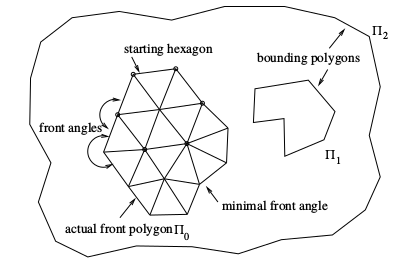
\includegraphics[scale=0.7]{images/hartmann1.png}
	\caption{Nociones básicas del algoritmo de triangulación.}
\end{figure}	
	
	\item[S1] Para cada punto del polígono $\Pi_0$ determinamos el ángulo del área aún por triangular. A estos ángulos los llamamos{ \em ángulos delanteros}.
	
	\begin{figure}[h]
		\centering
		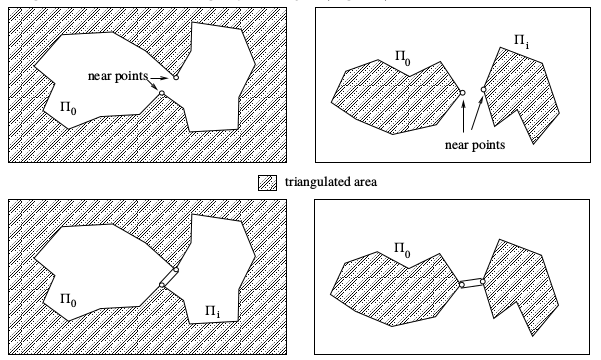
\includegraphics[scale=0.5]{images/hartmann2.png}
		\caption{Dividiendo y uniendo el polígono $\Pi_0$.}
	\end{figure}
	
	\item[S2] Revisamos si algún punto $p_i$ de $\Pi_0$ está cerca. Con cerca entendemos:
	\begin{itemize}
	\item Un punto de $\Pi_0$  distinto de $p_i$ y de su entorno.
	\item Un punto de cualquier otro polígono $\Pi_k$ distinto.
	\end{itemize}
	En el primer caso dividimos el polígono $\Pi_0$ en dos nuevos polígonos $\Pi_0$ y $\Pi_1$. En el segundo caso unimos los dos polígonos en uno nuevo al que llamaremos $\Pi_0$ y será nuestro nuevo polígono delantero actual.
	\item[S3] Determinar un punto $p_m$ del polinomio $\Pi_0$ con un ángulo delantero mínimo. Rodea $p_m$ por triángulos con ángulos cercanos a $\frac{\pi}{6}$. ELimina $p_m$ del polígono $\Pi_0$ e inserta los nuevos puntos en $\Pi_0$.
	\item[S4] Repite los pasos 1, 2 y 3 hasta que $\Pi_0$ consista sólo en tres puntos que generan un nuevo triángulo. Si aún queda algún polígono restante se convierte en el nuevo $\Pi_0$ y se repiten los pasos 1, 2 y 3. Una vez ya no queden más polígonos, habremos terminado y la triangulación estará completada.
\end{enumerate}

\subsubsection{El procedimiento \texttt{surfacepoint}}

Un paso fundamental del algoritmo es determinar el punto $p$ de la superficie que está cerca de un punto $q$ en un entorno de la superficie. El vector $q - p$ no ha de ser necesariamente perpenticular a la superficie. Debido a que casi todas las superficies pueden ser numéricamente implicitadas, daremos a solución para superficies implicitas.
\par Comenzamos con una superficie implícita $\Phi$ definida por una función $f(x) = 0$ para la cual su gradiente $\nabla f$ existe y no se anula para ningún punto de la superficie y un punto $q$ en un entorno de la superficie.
\par El siguiente procedimiento calcula un punto de la superficie $p$, un normal y dos vectores tangentes al punto $p$.

\begin{enumerate}
	\item \begin{itemize}
		\item $u_0 := q$
		\item Repetir $u_{k+1} := u_k - \frac{f(u_k)}{\nabla f(u_k)^2} \nabla f(u_k)$ hasta que $\| u_{k+1} - u_k \|$ es sficientemente pequeño.
		\item $p := u_{k+1}$ 
\end{itemize}		
	\item Definimos el normal a la superficie en $p$ como $n := \frac{\nabla f(p)}{\| \nabla f(p) \|}$.
	\item Para los vectores tangentes: \begin{itemize}
		\item $t_1 := \frac{1}{\| \sqrt{n_x^2 + n_y^2} \|} (n_y, -n_x, 0)$ si $n_x > 0.5$ ó $n_y > 0.5$.
		\item En otro caso elegimos $t_1 := \frac{1}{\| \sqrt{n_x^2 + n_z^2} \|} (-n_z, 0, n_x)$.
		\item $t_2 := n \times t_1$
	\end{itemize}
\end{enumerate}

\subsubsection{La estructura}

Para la construcción de los triángulos necesitamos un paso de longitud $\delta_t > 0$ qie es aproximadamente la longitud de las aristas.
\par Para cada putno $p_i$ guardamos la siguiente información:
\begin{itemize}
	\item Las coordinadas.
	\item El normal y los tangentes a la superficie en $p_i$ tales que son ortonormales entre sí.
	\item El ángulo delantero de $p_i$ si es un punto delantero de $\Pi_0$.
	\item La variable booleana \texttt{angle\_changed} con \texttt{angle\_changed = true} si el ángulo delantero cambió y tiene que ser recalculado.
	\item La variable booleana \texttt{border\_point}, con el valor \texttt{true} si el punto $p_i$ es en el borde de la triangulación y debería ser ignorado para futuros cálculos.
\end{itemize}

Los triángulos serán numerados de forma consecutiva. Para cada triángulo guardaremos el valor numérico de sus vértices.

\subsubsection{S0}

Sea $s$ un punto inicial en un entorno de la superficie. Entonces \texttt{surfacepoint} nos determina el primer punto $p_1$ de la triangulación y el sistema ortonormal $n_1, t_{11} \text{ y } t_{12}$. El resto de puntos $P_2, \dotso, p_7$ son el resultado de aplicar \texttt{surfacepoint} a:

$$q_{i+2} = p_1 + \delta_t cos\left(\frac{i \pi}{3}\right)t_{11} + \delta_t sen\left(\frac{i\pi}{3}\right)t_{12} \hspace{1cm} i = 0, \dotso, 5$$

Ya hemos obtenido los primeros seis triángulos.

\subsubsection{S1}

Si un punto $p_{0i}$ del polígono delantero $\Pi_0 = (p_{01}, \dotso, p_{0N_0})$ acaba de ser incluido o un punto cercano a $p_{0i}$ es un nuevo punto, entonceces es necesario recalcular elángulo delantero $\omega$ del punto $p_{0i}$. Sea:

\begin{itemize}
	\item $v_1 := p_{0,i-1}$ si $i>1$ ó $v_1 := p_{0N_0}$ si $i=1$.
	\item $v_2 := p_{0,i+1}$ si $i<N_0$ ó $v_2 := p_{01}$ si $i=N_0$.
	\item $(\xi_1,\eta_1,\zeta_1)$ y$(\xi_2,\eta_2,\zeta_2)$ las coordenadas de $v_1$ y $v_2$, respectivamente, en el sistema local ortonormal $n, t_1$ y $t_2$ en el punto $p_{0i}$.
	\item $\omega_i$ el ángulo polar de $(\xi_i, \eta_i)$. 
\end{itemize}

Entonces el ángulo delantero en el punto $p_{0i}$ es $\omega = \omega_2 - \omega_1$ si $\omega_2 \geq \omega_1$ ó $\omega = \omega_2 - \omega_1 + 2\pi$ en caso contrario.

\subsubsection{S2}

Para prevenir el solapamiento de nuevos triaángulos sobre los ya existentes comprobaremos:

\begin{itemize}
\item Las distancias dos a dos de los puntos que componen $\Pi_0$. Si hay puntos $p_{0i}$ y $p_{0j}$, con $i<j$, que no son vecinos, ni vecinos de vecino y $\| p_{0i} - p_{0j} \| < \delta_t$ entonces $\Pi_0$ se separa en dos polígonos.
\item Las distancias de puntos de $\Pi_0$ a puntos del resto de polígonos $\Pi_k$. Si hay puntos $p_{0i} \in \Pi_0$ y $p_{mj} \in \Pi_m$ tales que $\| p_{0i} - p_{mj} \| < \delta_t$, entonces los polígonos $\Pi_0$ y $\Pi_m$ se unen.
\end{itemize}

\begin{figure}[h]
\centering
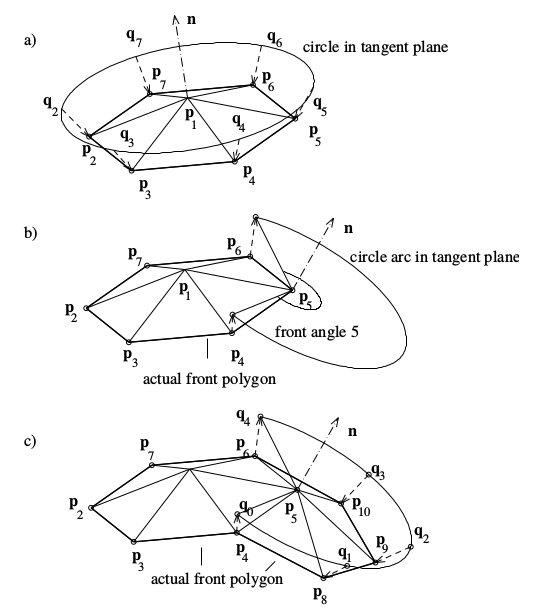
\includegraphics[scale=0.6]{images/hartmann3.png}
\caption{Los primeros pasos del algoritmo.}
\end{figure}

\subsubsection{S3}

Sea $p_{0m}$ un punto de $\Pi_0$  con un ángulo delantero mínimo $\omega$. Completamos la triangulación en $p_{0m}$ de la siguiente manera:

\begin{figure}[h]
\centering
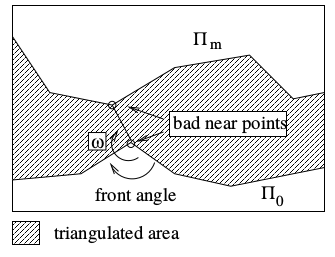
\includegraphics[scale=0.5]{images/hartmann4.png}
\caption{Puntos cercanos \textit{malos} y su detección.}
\end{figure}

\begin{enumerate}
\item Determinamos los vecinos $v_1$ y $v_2$ de $p_{0m}$.
\item Determinamos el número $n_t$ de triángulos que van a ser generados:
$$n_t := \mathtt{trunc}\left( \frac{3\omega}{\pi} \right) + 1 \hspace{1cm} \Delta \omega := \frac{\omega}{n_t}$$
Corrección de $\Delta \omega$ para casos extremos:
\begin{itemize}
\item Si $\Delta \omega < 0.8$ y $n_t > 1$ entonces $n_t \to n_t - 1$ y $\Delta \omega = \frac{\omega}{n_t}$.
\item Si $\Delta \omega < 0.8$, $n_t = 1$ y $\| v_1 - v_2 \| > \frac{5}{4} \delta_t$ entonces $n_t = 2$ y $\Delta \omega \to \frac{\Delta \omega}{2}$.
\item Si $\omega < 3$ y $\| v_1 - p_{0m} \| \leq \frac{1}{2} \delta_t$ (ó $\| v_1 - p_{0m} \| \leq \frac{1}{2} \delta_t$) entonces $n_t = 1$.
\end{itemize}

\begin{figure}[h]
\centering
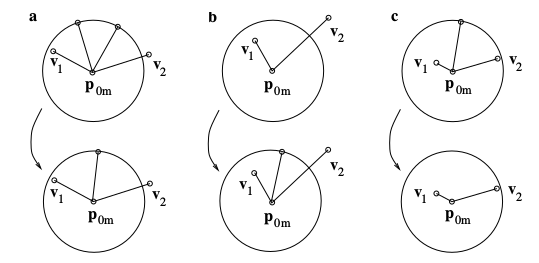
\includegraphics[scale=0.5]{images/hartmann5.png}
\caption{Correcciones de los casos extremos.}
\end{figure}

\item Generamos los triángulos:
\par Si $n_t = 1$ entonces tenemos un nuevo triángulo $(v_1, v_2, p_{0m})$ en otro caso sean $q_0$ y $q_{n_t}$ las proyecciones ortogonales de $v_1$ y $v_2$ en el plano tangente en el punto $p_{0m}$ y sea $q_i$ el resultado de una rotación de ángulo $i \Delta \omega$ alrededor del normal a la superficie en $p_{0m}$ aplicada a $p_{0m} + \delta_t \frac{q_0 - p_{0m}}{\| q_0 - p_{0m} \|}$. Aplicando el procedimiento \texttt{surfacepoint} a $q_i$ obtendremos nuevo puntos $p_{N+i}$ $i = 1, \dotso, n_t -1$, donde $N$ es el total de puntos existentes hasta el momento, y $n_t$ nuevos triángulos.
\item Renovamos el polígono $\Pi_0$:
\par Borramos el punto $p_{0m}$ y, si $n_t > 1$, insertamos en su posición los nuevos puntos $p_{N+1}, \dotso, p_{N+n_t-1}$. Todas las variables booleanas tiene el valor \texttt{true} para asegurarnos de que los nuevos cálculos se realizan.
\end{enumerate}

\subsection{Ejemplos de superficies trianguladas}

\subsubsection{Esfera}

Triangulación de la esfera $x^2 + y^2 + z^2 - 4 = 0$ comenzando por el punto $(1,1,1)$ y paso de longitud $\delta_t = 0.3$. La siguiente imagen muestra los primeros cuatro polígonos delanteros y la situación tras 101 y 1531 triángulos. La triangulación total involucra 1534 triángulos.
\[\]
\begin{figure}[h]
\centering
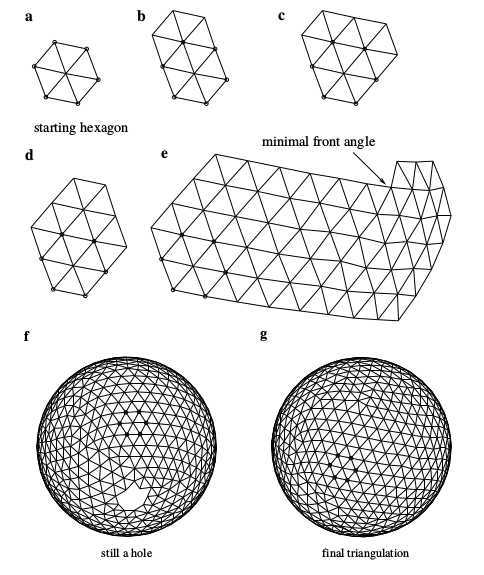
\includegraphics[scale=0.7]{images/hartmann6.png}
\caption{Poceso de triangulación de la esfera.}
\end{figure}

\newpage
\subsubsection{Cilindro}

Triangulación del cilindro $x^2 + y^2 - 1 = 0$ comenzando por el punto $(1,0,0)$ y paso de longitud $\delta_t = 0.2$. 
\[\]
\begin{figure}[h]
\centering
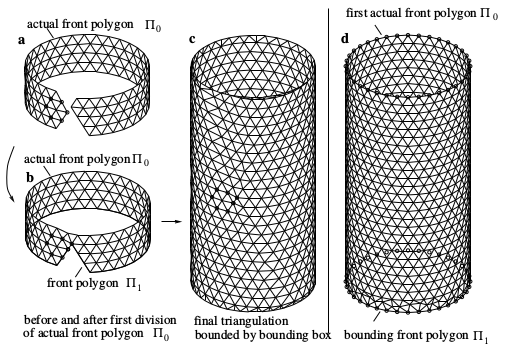
\includegraphics[scale=0.8]{images/hartmann7.png}
\caption{Poceso de triangulación del cilindro.}
\end{figure}

\newpage
\subsubsection{Toro}

Triangulación del cilindro $(x^2+y^2+z^2+0.8775) - 4(x^2+y^2)=0$ comenzando por el punto $(1,0,0.5)$ y paso de longitud $\delta_t = 0.1$.
\[\]

\begin{figure}[h]
\centering
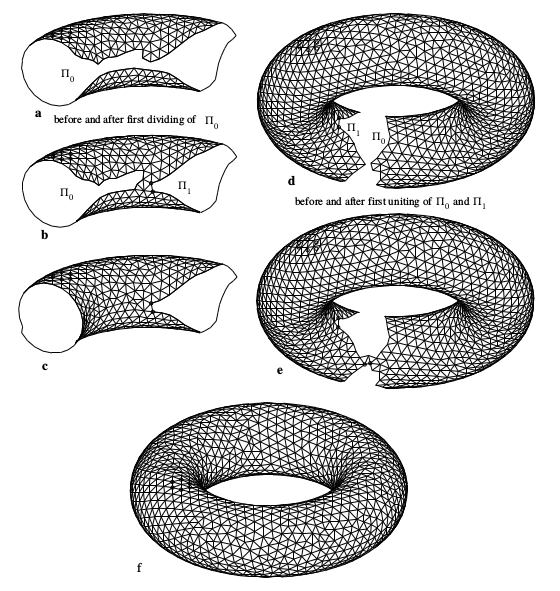
\includegraphics[scale=0.7]{images/hartmann8.png}
\caption{Poceso de triangulación del toro.}
\end{figure}

\subsection{Ray Tracing en superficies implícitas}